\chapter{Model Architecture and Experiments}
\phantomsection
\label{ch:experiments}

\section{Experimental Environment and Tools}
\label{sec:environment}
All experiments in this study were conducted on a high-performance workstation running 
Ubuntu 20.04 LTS. The system was equipped with dual NVIDIA RTX 4090 GPUs, each with 
48 GB of VRAM, and 128 GB of system RAM, ensuring ample memory and computational power 
for training large-scale deep learning models efficiently.

The models were implemented using the PyTorch deep learning framework, with integration of the Hugging Face Transformers library for state-of-the-art model architectures such as TrOCR. GPU acceleration was enabled via CUDA, allowing for fast and parallelized training across the two GPUs.

For experiment tracking and metric logging, MLflow was used. It captured key training 
and evaluation metrics such as character error rate (CER), word error rate (WER), 
training loss, and validation loss in real-time. This facilitated better experiment 
management and reproducibility, especially when comparing multiple model versions or 
hyperparameter configurations.



\section{Model Architecture and Configuration}
\label{sec:architecture}
Details of the model architectures and configurations used in the OCR system.

\subsection{CRAFT for Text Detection}
\label{subsec:craft}

For the text detection stage, we adopted the Character Region Awareness for Text 
Detection (CRAFT) model, which is well-regarded for its ability to detect text at 
the character level rather than relying solely on word-level bounding boxes. 
CRAFT produces dense predictions of character regions and affinity scores, 
enabling it to localize irregular and closely spaced text lines—an essential 
requirement for handling complex scripts like Khmer.

The CRAFT model architecture consists of a VGG16-based backbone followed by a series 
of convolutional layers to produce two output maps:
\begin{itemize}
\item A \textbf{region score map}, indicating the likelihood of each pixel belonging 
to a character region.
\item An \textbf{affinity score map}, capturing the spatial relationships between 
adjacent characters to form text lines.
\end{itemize}

In this study, we fine-tuned a pretrained CRAFT model on a custom Khmer dataset 
composed of synthetic and real-world scene text images. We applied data augmentation 
techniques such as rotation, scaling, blurring, and illumination changes to increase 
the model's robustness. The input images were resized to a fixed height of 768 pixels 
while preserving the aspect ratio.

We used the official implementation of CRAFT with some modifications to better support
Khmer character characteristics, such as tight spacing, stacked glyphs, and diacritic 
marks. The model was trained using Adam optimizer with a learning rate of 1e-4 and batch 
size of 16. Early stopping and validation-based checkpointing were employed to 
prevent overfitting.

The output of the CRAFT detector was then passed to the text recognition 
model (TrOCR), enabling a two-stage pipeline for accurate and end-to-end 
Khmer text reading in natural scenes.

\begin{figure}[ht]
    \centering
    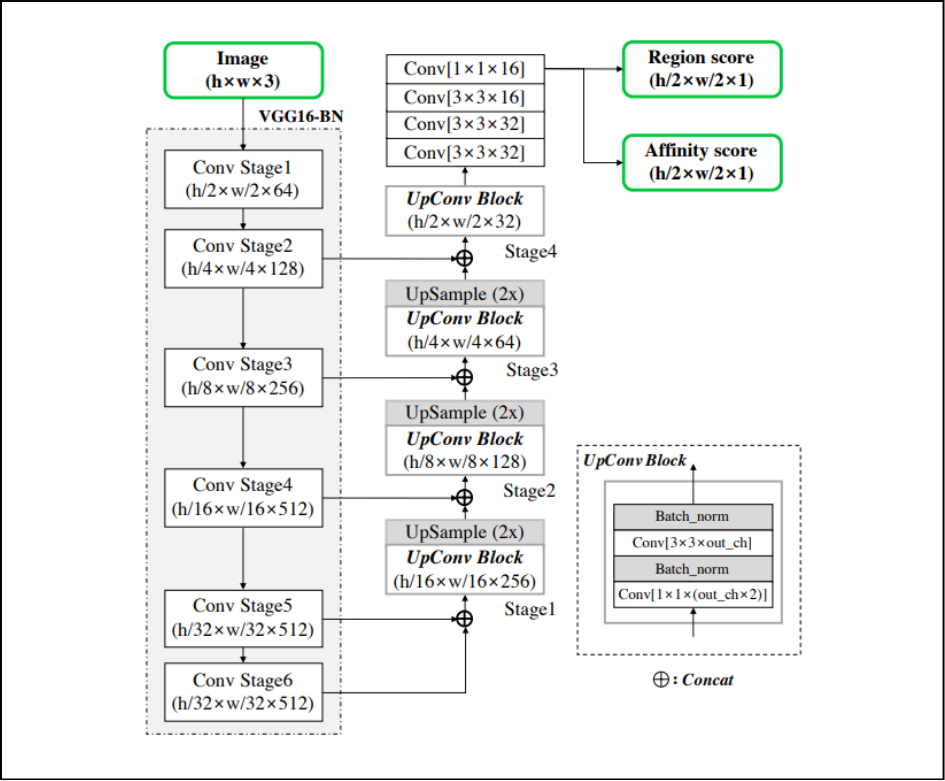
\includegraphics[width=\textwidth]{figures/craft_model.png}
    \caption{Illustration of the CRAFT model architecture used for text detection. \cite{baek2019craft}}
    \label{fig:craft-model}
\end{figure}


\subsection{TrOCR for Text Recognition}
\label{subsec:trocr}

For the text recognition component of the pipeline, we used the \textbf{TrOCR} model, 
a transformer-based OCR system proposed by Microsoft Research. TrOCR stands for 
\textit{Transformer-based Optical Character Recognition}, and it integrates a vision 
encoder with a language decoder in a unified encoder-decoder (Seq2Seq) architecture, 
following the structure of the Vision Transformer (ViT) and pre-trained language models 
like BART.

The TrOCR model takes the cropped text-line image detected by CRAFT and processes it through a \textbf{ViT-based encoder}, which extracts rich visual features. These features are then passed to the \textbf{transformer decoder}, which generates the text sequence token-by-token, using cross-attention to focus on relevant image features while decoding. This allows the model to handle complex scripts like Khmer with better accuracy and context-awareness.

We fine-tuned the base version of TrOCR using the Hugging Face \texttt{transformers} library on our custom synthetic Khmer dataset. During training, we tracked key metrics such as Character Error Rate (CER) and Word Error Rate (WER) using MLflow. The model demonstrated strong generalization across different fonts and text conditions, benefiting from both large-scale pretraining and our domain-specific fine-tuning.

\begin{figure}[ht]
    \centering
    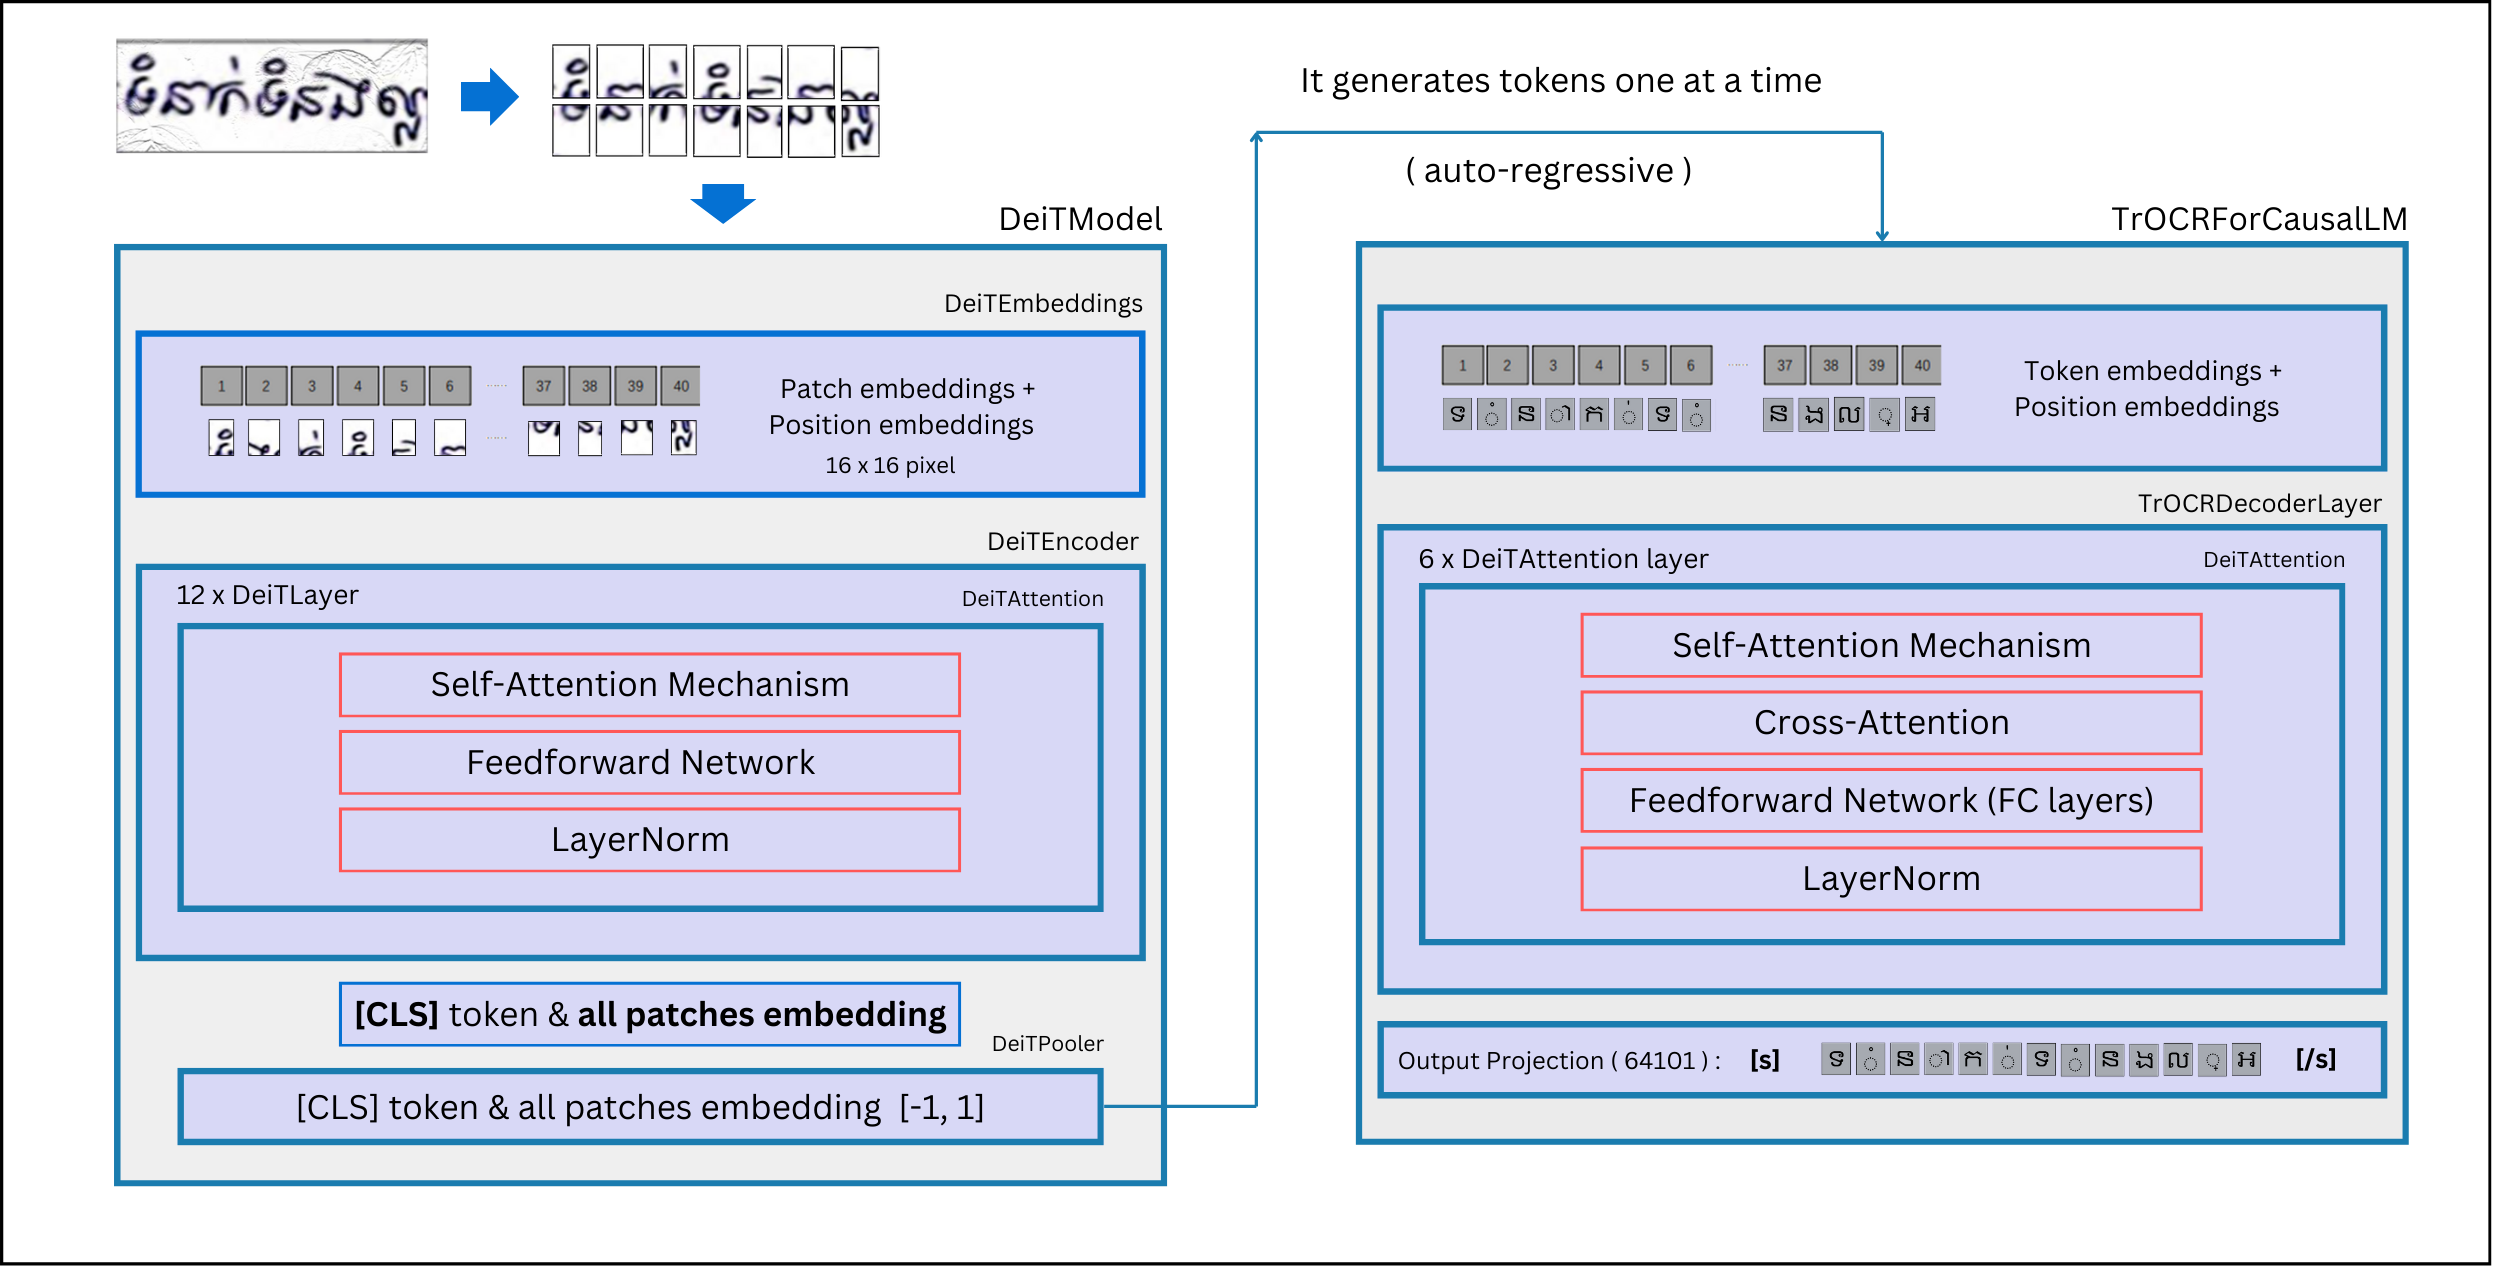
\includegraphics[width=\textwidth]{figures/trocr_model.png}
    \caption{Illustration of the TrOCR model architecture used for text recognition.}
    \label{fig:trocr-model}
\end{figure}


\section{Training Methodology}
\label{sec:training}
This section delves into the training strategies and processes employed to optimize 
the performance and accuracy of the OCR models. We describe the fine-tuning procedures 
for both the CRAFT text detector and TrOCR text recognizer, as well as the key 
hyperparameters and metrics used to evaluate their performance. Additionally, we 
present a discussion on the importance of robust training and the approaches taken 
to ensure the models generalize well across different fonts, text conditions, and 
domains.



\subsection{Fine-tuning Configuration for CRAFT}
\label{subsec:craft-training}

The CRAFT model was fine-tuned on a custom Khmer text dataset using weak supervision, 
leveraging the strengths of annotated real images. During 
training, we applied a range of augmentations to improve robustness against font 
variations, noise, and other distortions. To further enhance the model's generalization 
abilities, we employed techniques such as random cropping, flipping, and rotation to 
increase the diversity of the training data. Additionally, we used a combination of 
contrastive learning and adversarial training to improve the model's ability to 
discriminate between different characters and fonts. Finally, we used transfer learning 
to adapt the model to the Khmer language by fine-tuning it on a small dataset of 4000 
manually annotated bounding boxes. This dataset was carefully curated to capture the 
unique characteristics of the Khmer script, such as its complex diacritic marks and 
ligatures. The most important configuration values for training the CRAFT model are 
summarized in Table~\ref{tab:craft-training-config}, including the training mode, 
backbone architecture, pre-trained weights, loss function, normalization parameters, 
and optimization hyperparameters. These settings are crucial for achieving optimal 
performance on the Khmer text dataset.

\noindent
\textbf{Data Augmentation:} During training, the following augmentations were applied:
\begin{itemize}
    \item \textbf{Random rotation:} Up to 20° (enabled).
    \item \textbf{Random cropping:} Variable scale and aspect ratio.
    \item \textbf{Horizontal flipping:} Enabled.
    \item \textbf{Color jittering:} Adjustments in brightness, contrast, saturation, and hue (each set to 0.2).
\end{itemize}



\begin{table}[ht]
\centering
\begin{tabular}{|p{0.4\linewidth}|p{0.55\linewidth}|}
\hline
\textbf{Parameter} & \textbf{Value} \\
\hline
Training mode & \texttt{weak\_supervision} \\
Backbone architecture & VGG \\
Use of SynthText & False \\ 
Real dataset & \texttt{custom} \\
Pretrained weights & \texttt{CRAFT.pth} \\
Batch size & 5 \\
Training iterations & 0 to 10,000 \\
Evaluation interval & Every 500 iterations \\
Learning rate & 0.0001 \\
Learning rate decay step & 7,500 \\
Decay rate ($\gamma$) & 0.2 \\
Weight decay & 0.00001 \\
Mixed precision (AMP) & Enabled \\
Loss function type & 2 \\
Negative ratio & 0.3 \\
Minimum negative samples & 5,000 \\
Output image size & 768 \\
Normalization mean & [0.485, 0.456, 0.406] \\
Normalization std (variance) & [0.229, 0.224, 0.225] \\
Region enlargement factor & [0.5, 0.5] \\
Affinity enlargement factor & [0.5, 0.5] \\
Gaussian kernel init size & 200 \\
Gaussian sigma & 40 \\
\hline
\end{tabular}
\caption{Key configuration parameters for training the CRAFT model on a custom Khmer dataset 
using weak supervision. The parameters include the training mode, backbone architecture, 
dataset, batch size, training iterations, evaluation interval, learning rate, learning rate decay, 
weight decay, mixed precision, loss function type, negative ratio, minimum negative samples, 
output image size, normalization mean and standard deviation, region and affinity enlargement 
factors, Gaussian kernel initialization size, and Gaussian sigma.}
\label{tab:craft-training-config}
\end{table}


\subsection{Customizing TrOCR Processor}
\label{subsec:customizing-trocr-processor}
To make the TrOCR model understand Khmer tokens, we customized the processor of the TrOCR 
model from Microsoft. We collected unique Khmer and English tokens and then modified the 
processor to encode text to IDs and decode IDs to text. After customizing the processor, 
everything looked fine, and we could start fine-tuning.

\subsection{Fine-tuning TrOCR Model}
\label{subsec:fine-tuning-trocr-model}
For the TrOCR model, we selected the base model because we were working with a multilingual 
dataset. We wanted the model to have a large parameter size, so we chose the base model for 
this task.

After experimenting with different hyperparameters, we found the desired results. Here are the 
desired hyperparameters: batch size = 1024, learning rate = 0.0001, epoch = 2, dataset = 3.5 
million images. We chose a batch size of 1024 because we wanted the model to generalize well. 
This is a very important hyperparameter because we used to train with 8, 16, 32, 128, 256, 
but it was not generalizing as expected; it was really weak to overfitting. That's why we 
chose 1024.

\begin{figure}[ht]
    \centering
    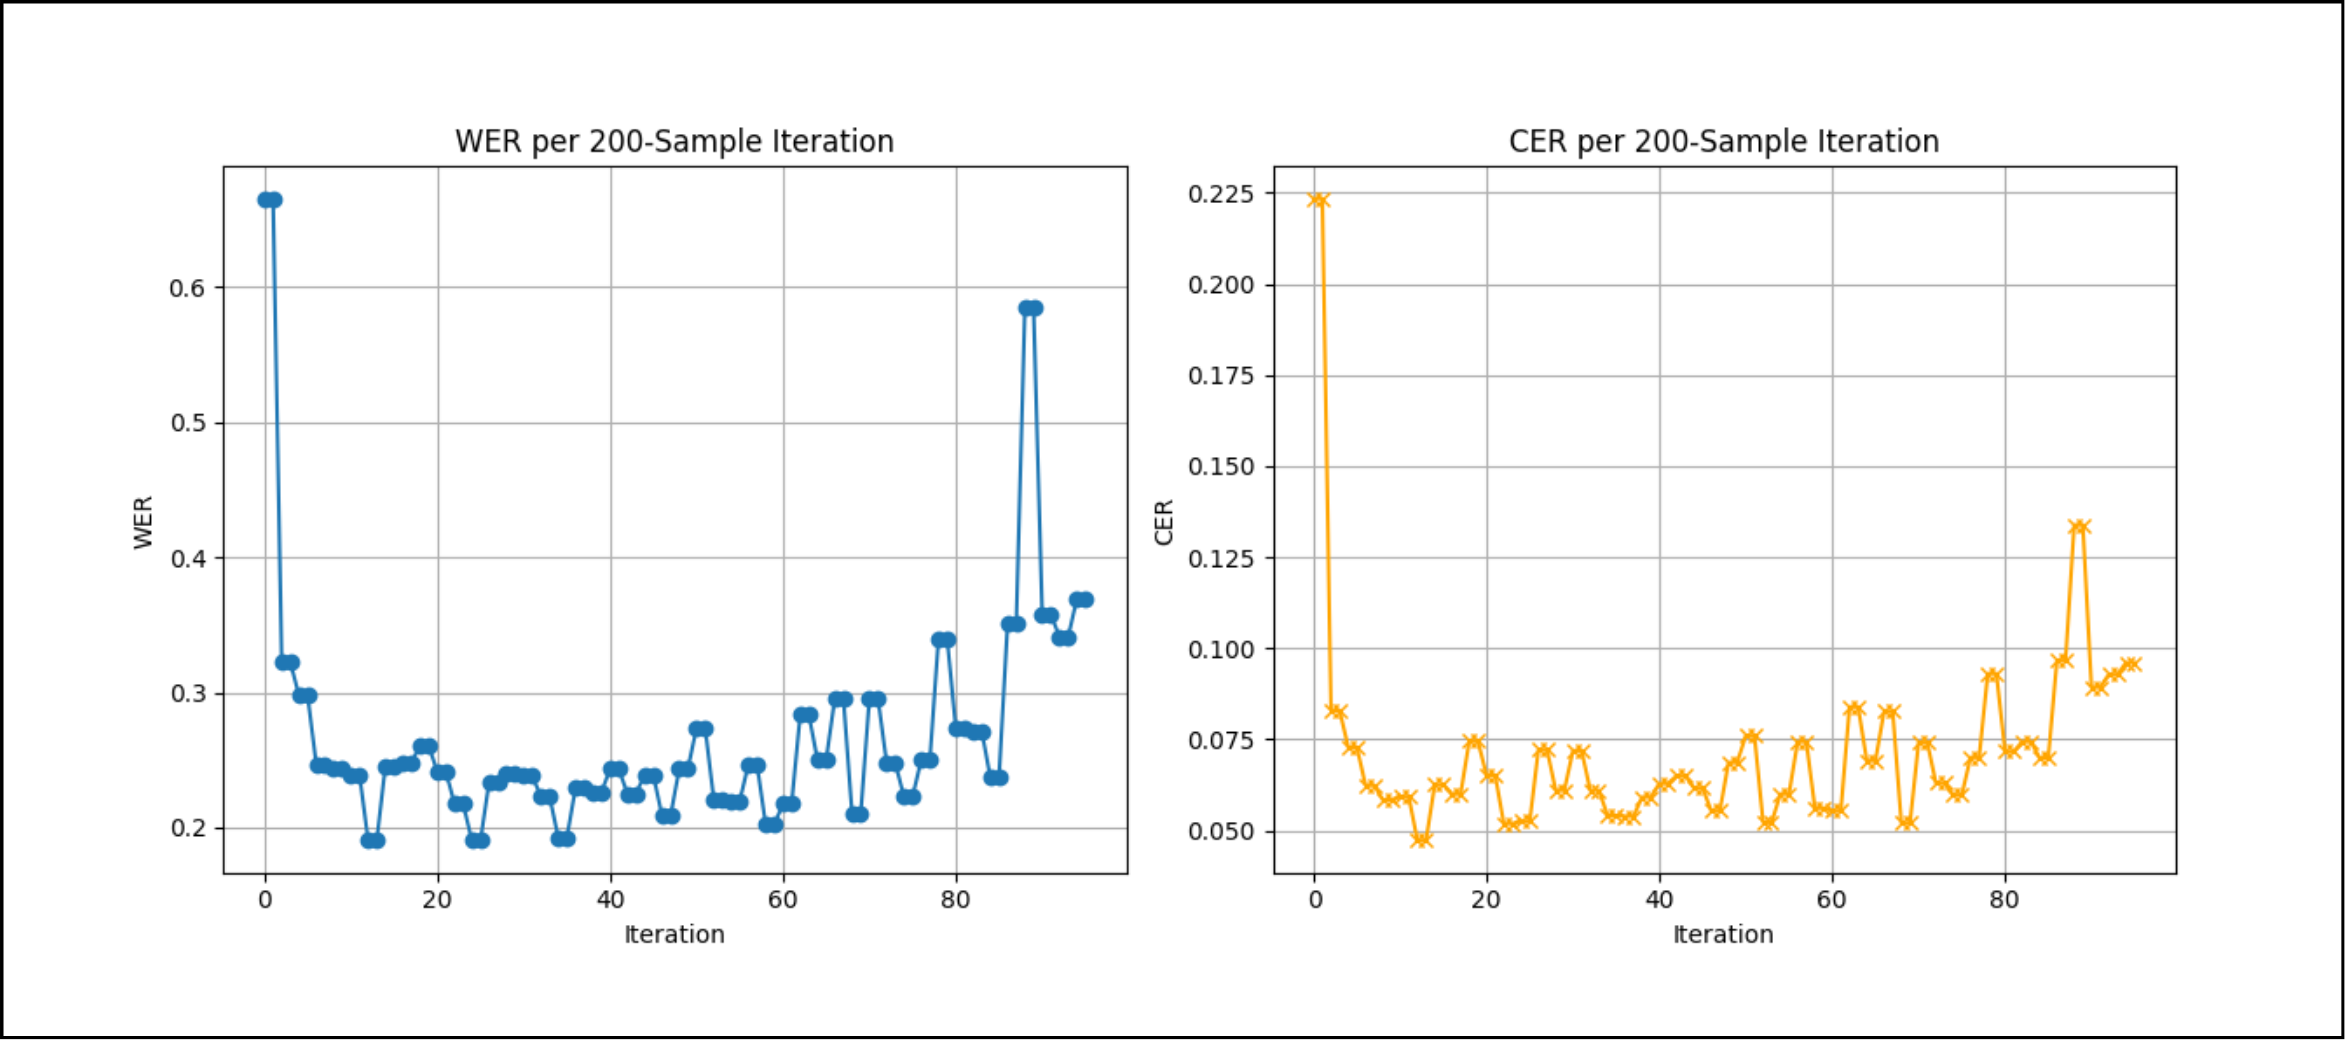
\includegraphics[width=\textwidth]{figures/trocr_overfitting_v1.png}
    \caption{Training and validation loss curves for TrOCR model with batch size 8.}
    \label{fig:trocr-overfitting}
\end{figure}

The graph above illustrates a clear case of overfitting in our TrOCR model training. 
We initially trained the model with a batch size of 8 on our dataset of 3.5 million images. 
As shown in the figure, while the training loss (blue line) continues to decrease, 
the validation loss (orange line) starts to increase, indicating that the model is overfitting 
to the training data. This overfitting occurs because the batch size of 8 is too small relative 
to our large dataset size of 3.5 million images. With such a small batch size, the model learns 
very specific patterns from the training data rather than generalizing well to unseen data. 
This is why we decided to increase the batch size to 1024, which helped improve the model's 
generalization capabilities and reduce overfitting.

\begin{figure}[ht]
    \centering
    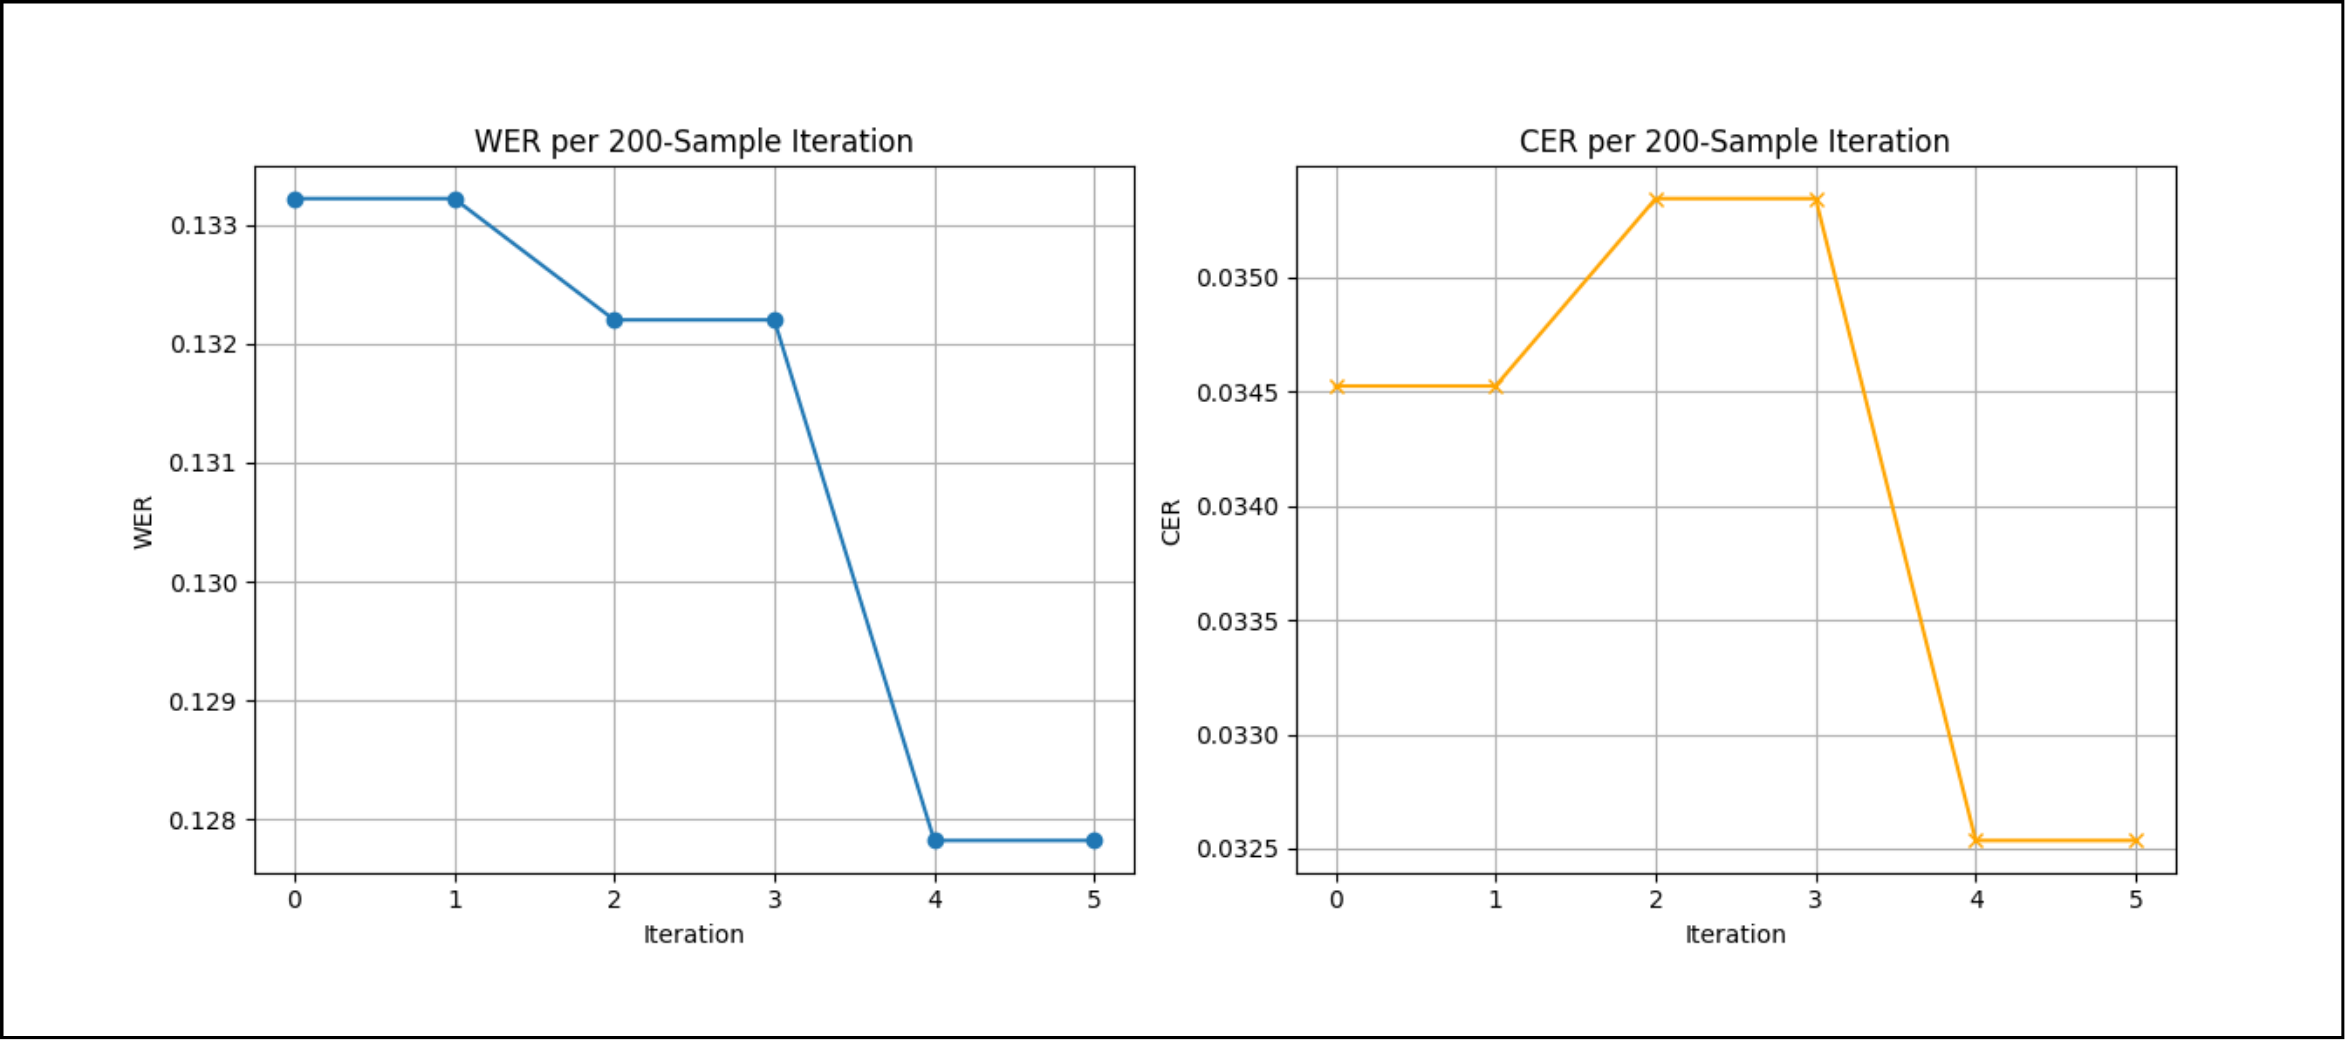
\includegraphics[width=\textwidth]{figures/trocr_fine_tuning.png}
    \caption{Training and validation metrics for TrOCR model with batch size 1024, 
    showing Character Error Rate (CER) and Word Error Rate (WER) over training steps. 
    The model demonstrates excellent performance from early training steps, with CER quickly 
    reaching around 0.03 and WER staying below 0.12. This rapid convergence indicates effective 
    learning, likely due to leveraging the pretrained weights from previous training. 
    The larger batch size of 1024 contributes to better generalization compared to smaller batch sizes.}
    \label{fig:trocr-fine-tuning}
\end{figure}

The figure above demonstrates the effectiveness of our fine-tuning approach with a batch size of 1024. 
The model shows remarkable performance from the early stages of training, with the Character 
Error Rate (CER) quickly stabilizing around 0.03 and the Word Error Rate (WER) maintaining 
values below 0.12. This rapid convergence to good performance metrics can be attributed to 
two main factors: (1) the utilization of pretrained weights from previous training iterations, 
which provides a strong foundation for the model, and (2) the larger batch size of 1024, which 
helps the model learn more robust features and generalize better to unseen data. The stable 
performance across both training and validation sets indicates that the model has achieved a 
good balance between learning and generalization, avoiding the overfitting issues we 
encountered with smaller batch sizes.


\section{Evaluation Metrics}
\label{sec:metrics}
Metrics used to evaluate the performance of the OCR system.

\subsection{Detection Metrics (Precision, Recall)}
\label{subsec:detection-metrics}
Text detection evaluation using precision and recall metrics.

\begin{figure}[ht]
    \centering
    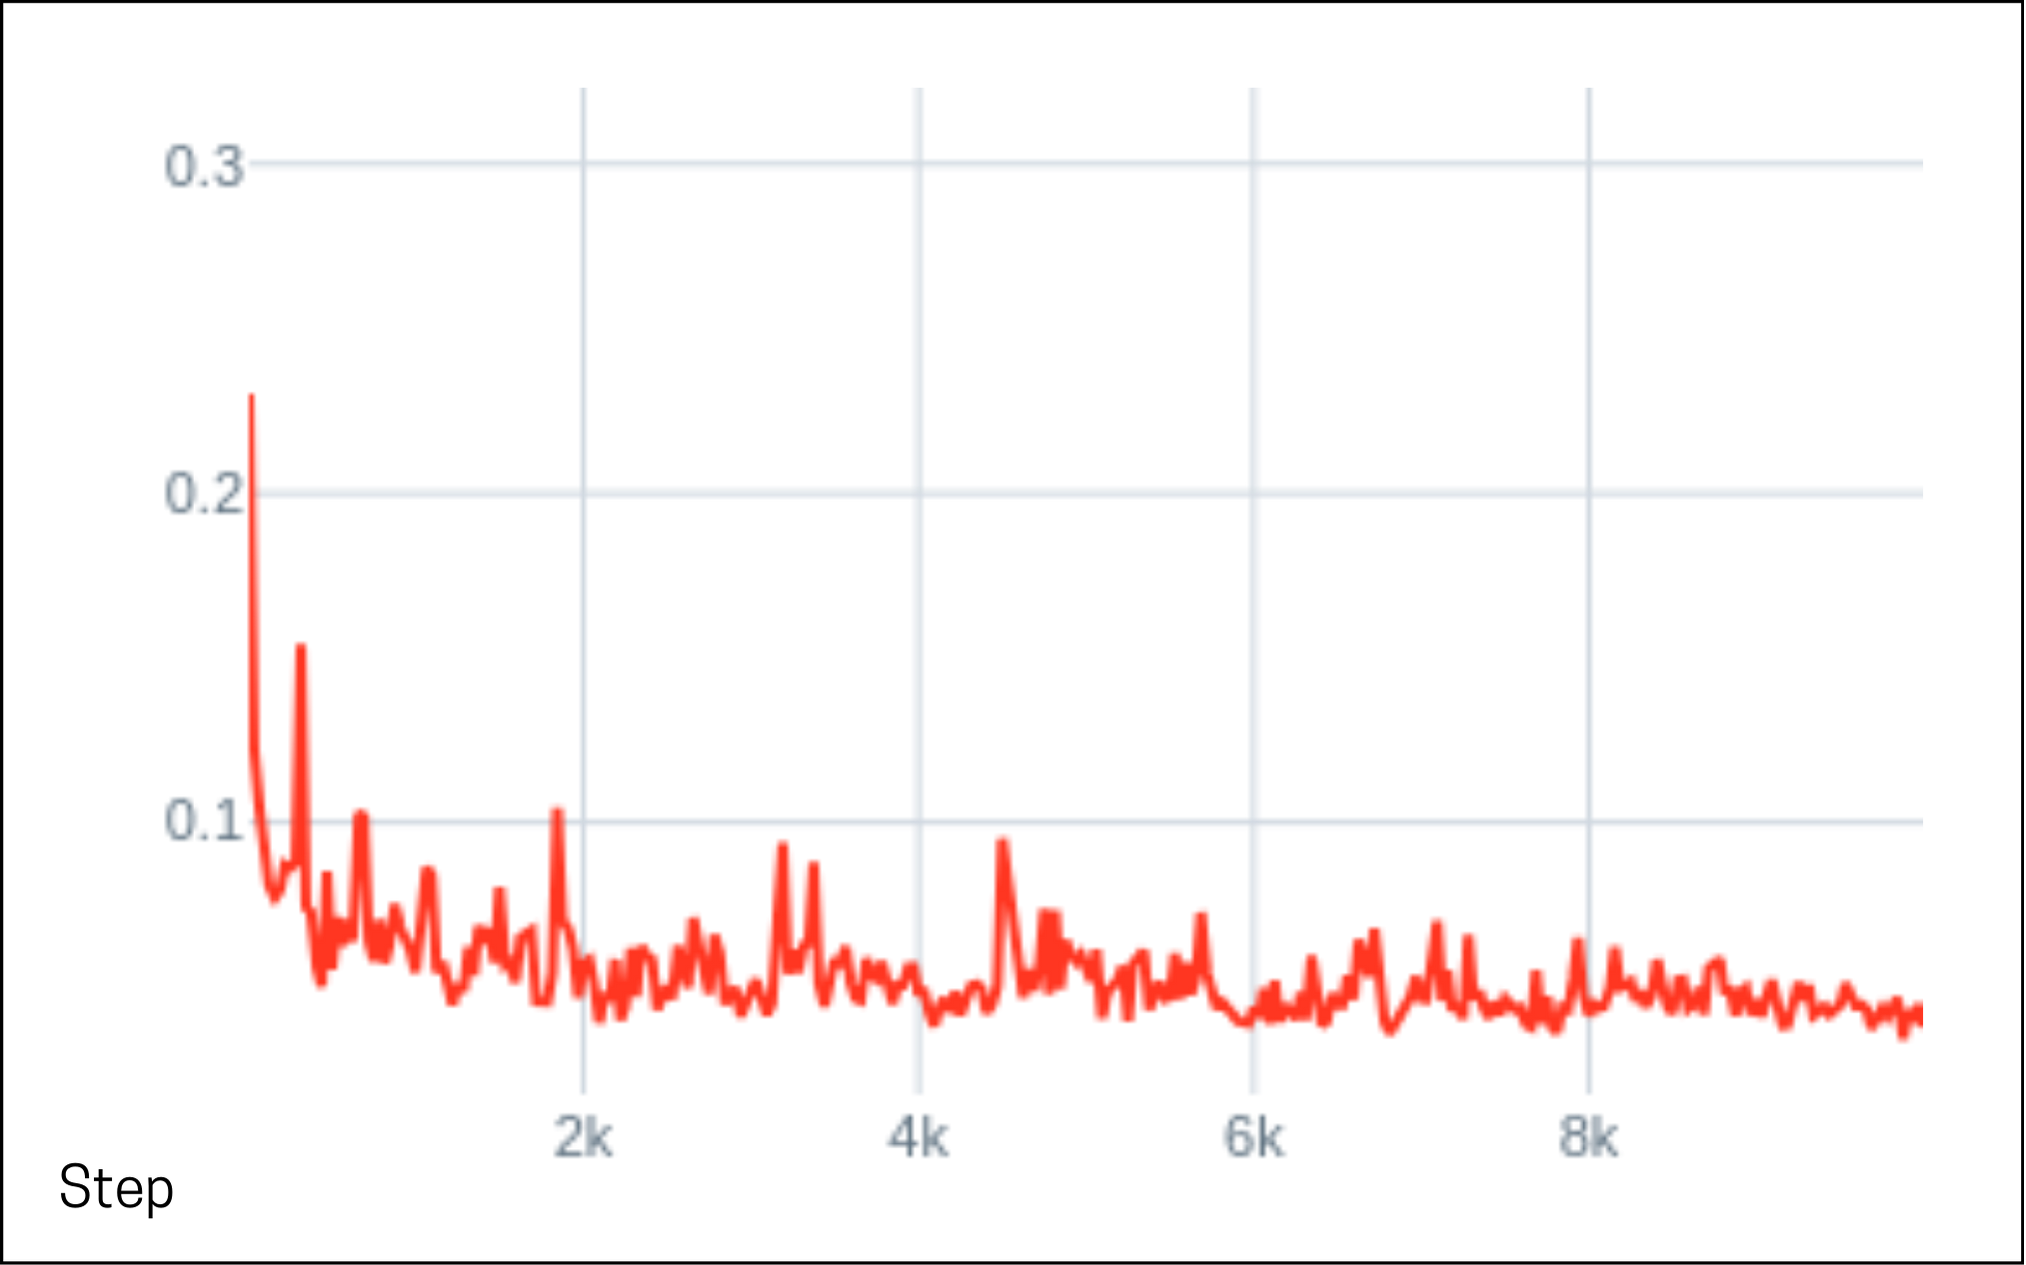
\includegraphics[width=\textwidth]{figures/mean_loss_craft.png}
    \caption{Illustration of the mean loss during CRAFT model training, showing the performance 
    improvement over time. The mean loss decreased rapidly in the first 500 iterations, 
    indicating that the model was able to quickly adapt to the training data. The loss then 
    continued to decrease at a slower rate until around 2,000 iterations, at which point 
    the model's performance began to plateau. After 2,000 iterations, the loss remained 
    relatively stable, indicating that the model had converged and was no longer improving.}
    \label{fig:mean-loss-craft}
\end{figure}

\begin{figure}[ht]
    \centering
    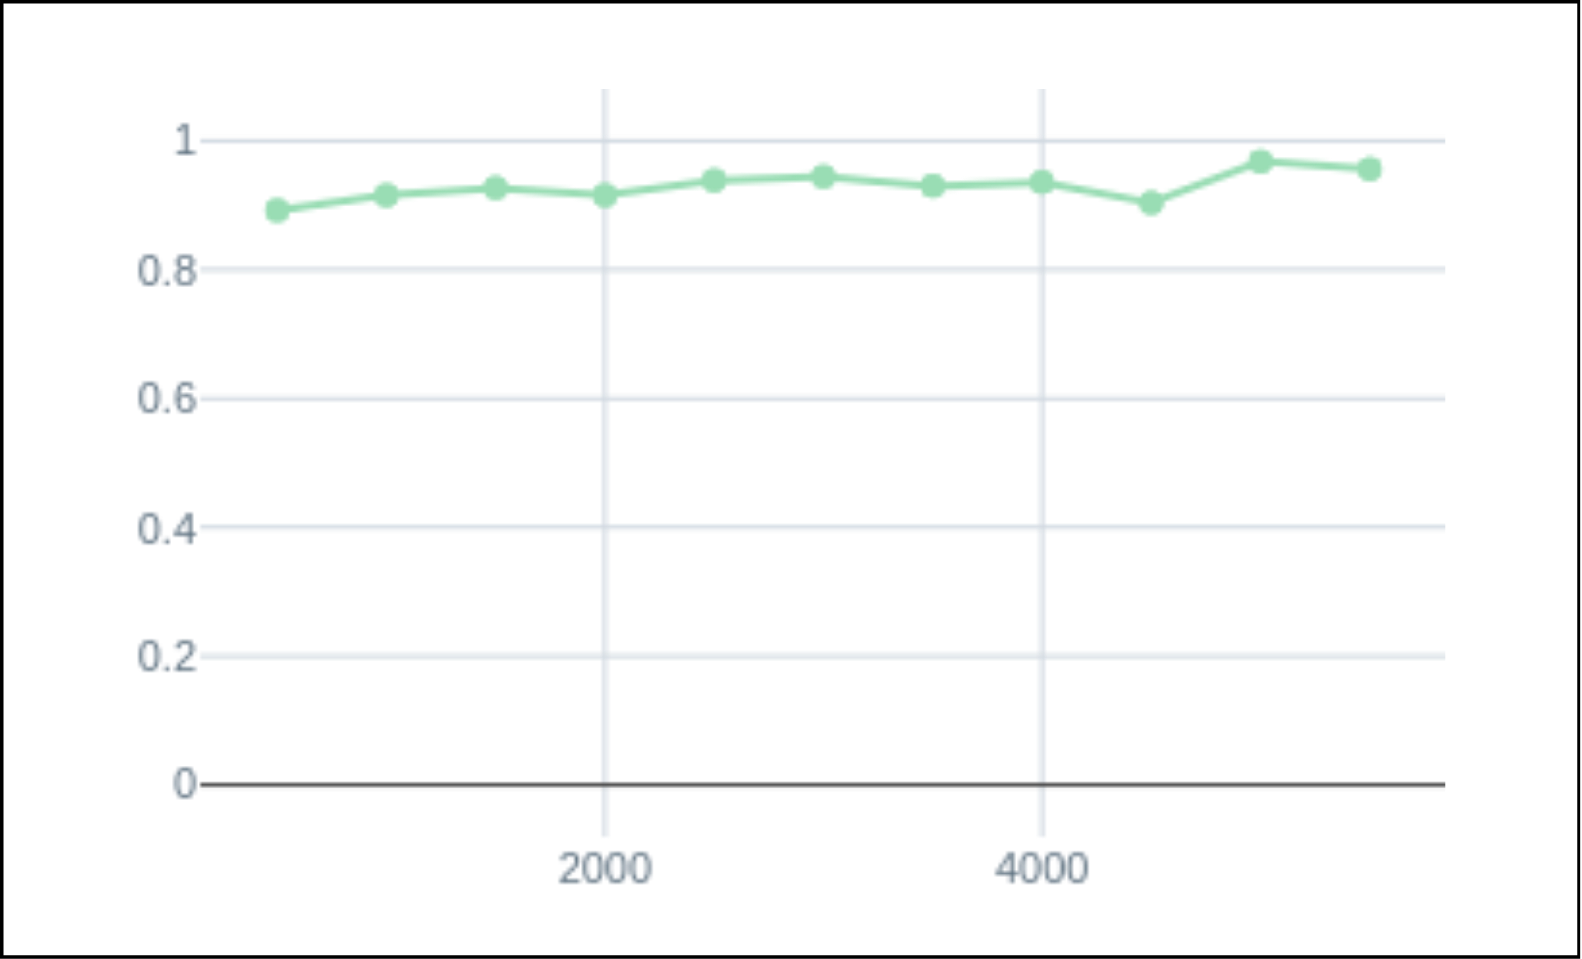
\includegraphics[width=\textwidth]{figures/iou_craft.png}
    \caption{Illustration of the intersection over union (IOU) vs. recall performance of the CRAFT model 
    during text detection evaluation. The IOU is a measure of how well the bounding box predicted 
    by the model overlaps with the ground truth bounding box, while the recall measures how many of 
    the ground truth bounding boxes are detected by the model. The IOU-recall curve shows that the 
    model can detect most of the text regions with high accuracy. The model reaches a high recall of 
    90\% at an IOU of 0.5, indicating that the model is able to detect most of the text regions even 
    when the predicted bounding box is not perfectly aligned with the ground truth.}
    \label{fig:iou-recall-craft}
\end{figure}


\subsection{Recognition Metrics (Accuracy, CER, WER)}
\label{subsec:recognition-metrics}
For evaluating the text recognition performance of our TrOCR model, we employed three key metrics: Character Error Rate (CER), Word Error Rate (WER), and Accuracy. These metrics provide a comprehensive assessment of the model's recognition capabilities.

Character Error Rate (CER) measures the ratio of incorrect characters to the total number of characters in the ground truth text. It is calculated as:

\begin{equation}
    CER = \frac{S + D + I}{N}
\end{equation}

where $S$ is the number of substitutions, $D$ is the number of deletions, $I$ is the number of insertions, and $N$ is the total number of characters in the ground truth text.

Word Error Rate (WER) is similar to CER but operates at the word level. It measures the ratio of incorrect words to the total number of words in the ground truth text. WER is calculated as:

\begin{equation}
    WER = \frac{S_w + D_w + I_w}{N_w}
\end{equation}

where $S_w$ is the number of word substitutions, $D_w$ is the number of word deletions, $I_w$ is the number of word insertions, and $N_w$ is the total number of words in the ground truth text.

Accuracy is the complement of the error rate, representing the percentage of correctly recognized characters or words. For character-level accuracy:

\begin{equation}
    Accuracy_{char} = 1 - CER
\end{equation}

And for word-level accuracy:

\begin{equation}
    Accuracy_{word} = 1 - WER
\end{equation}

[Add Figure 1 here: A line plot showing the training and validation CER over epochs]
[Add Figure 2 here: A line plot showing the training and validation WER over epochs]
[Add Figure 3 here: A bar chart comparing final CER and WER scores across different test sets]

These metrics provide different perspectives on the model's performance. CER is more sensitive to character-level errors and is particularly useful for evaluating the model's ability to recognize individual characters accurately. WER, on the other hand, provides a higher-level view of the model's performance at the word level, which is often more relevant for practical applications. The accuracy metrics offer an intuitive way to understand the model's overall performance.
